\documentclass[letterpaper, 11pt]{article}

\usepackage{amsmath, amsthm, latexsym, amssymb, graphicx, bold-extra, mathrsfs, frcursive}
\usepackage[pdftex]{color}
\usepackage[T1]{fontenc}

% Simplifies margin settings
\usepackage{geometry}
\geometry{margin=1in}

% Puts list item indicators in bold; makes flush with previous margin
\renewcommand\labelenumi{\bf\theenumi.}
\renewcommand\labelenumii{\bf\theenumii.}
% setlength\leftmargini{1.4em}
\setlength\leftmarginii{1.4em}

% Flexibility for headers and footers
\usepackage{fancyhdr}
\pagestyle{fancyplain}
\fancyhf{} %clear all header and footer fields
\lhead{\bf \small Advanced Computer Networks \hspace*{\fill} Page \thepage}
\headsep 0.2in
\thispagestyle{empty}
\renewcommand{\headrulewidth}{0pt}
\renewcommand{\footrulewidth}{0pt}

\parindent 0in
\parskip 10pt
\setlength{\headheight}{20pt}

\title{ETH Zurich}

\begin{document}

%=======================================

\begin{center}
\Large \bf Advanced Computer Networks

\Large \bf Assignment 1: Network Principles

\large Submitted by Jinank Jain
\end{center}

\textbf{Solution 1}\\ \\
\textbf{Bandwidth-Delay Product:} \\
Mathematically it is defined as the product of bandwidth and round-trip delay time. Intuitively bandwidth-delay product of a transmission path defines the amount of data TCP should have within the transmission path at any one time, in order to fully utilize the available channel capacity.

Bandwidth-Delay product is usually most essential component of reliable communication as it will help to indicate congestion level in the network, thus it would be an important part of only those protocols which care about the reliability of the communication such as like TCP which uses it for TCP tuning because the protocol can only achieve optimum throughput if a sender sends a sufficiently large quantity of data before being required to stop and wait until a confirming message is received from the receiver, acknowledging successful receipt of that data.

Example of the system that has a large bandwidth-delay product are High-speed terrestrial network: 1 Gbit/s, 1 ms RTT, Mobile broadband (HSDPA): 6 Mbit/s, 100 ms RTT etc.

\bigskip

\textbf{Solution 2}\\ \\
\textbf{Part a} \\
In order to solve this part I make a simple assumption that there is no congestion and no packet loss. In the first RTT 1KB would be send, in the second 2KB would be sent for a total of 3KB. On round n, the amount of data sent during this round is given by the equation:

\[
    data_n = 
\begin{cases}
    2^{n-1} KB,& \text{if } x\le 10\\
    1024 KB,              & \text{otherwise}
\end{cases}
\]

In total of n iterations we would get the following

\[
    total\_data_n = 
\begin{cases}
    \sum_{i=0}^{n} 2^{i-1} KB,& \text{if } x\le 10\\
    1024*(n-10) + 1024 KB,              & \text{otherwise}
\end{cases}
\]
After analysis, we find that in 19 RTTs, a total of 10,239 KBytes (this is equal to 10 MBs - 1 KB, assuming that 1024 KB = 1 MB) have been sent and in 20 RTTs, a  total  of  11,263  KBytes  have  been  sent.   So  after  20  RTTs  the  file  would  be  sent completely.

\textbf{Part b} \\
Time to send the file would be:
\begin{center}
	Time = 20 RTTs * 100ms = 2 secs
\end{center}
And the effective throughput would be the following:
\begin{center}
Throughput = $\dfrac{10*8 Mb}{2 sec}$ Mbps \\
\leavevmode \newline
Throughput = 40 Mbps
\end{center}
\textbf{Part c} \\
If receive sizes are much larger then 1MB there will be no saturation and we can modify the above formula:
\begin{center}
	10*1024 KB = $\sum_{i=0}^{n} 2^{i-1}$ * 1KB
\end{center}

In this case the approximate value n would be 13.3 so after 14 RTT we could say that complete file would be transferred. So the new effective throughput would be:
\begin{center}
Throughput = $\dfrac{10*8 Mb}{1.4 sec}$ Mbps \\
\leavevmode \newline
Throughput = 57.14 Mbps
\end{center}
\bigskip

\textbf{Solution 3}\\ \\
According to the formula given in the question we can get the following parameters:
\begin{center}
Bandwidth = 1 Gbps \\
\leavevmode \newline 
File Size = 128 Mb \\
\leavevmode \newline 
Throughput = $\dfrac{128}{RTT + 0.128}$ Mbps
\end{center}

\textbf{Effect of RTT on file transfer:} \\
With increase in RTT throughput of the link would decrease and we would not be utilizing the link to the maximum extend on the other if RTT goes to zero we would reach near 1 Gbps which is close to maximum bandwidth that link could achieve.

\textbf{Graph of Throughput V/S RTT}
\begin{figure}[h!]
	\centering
    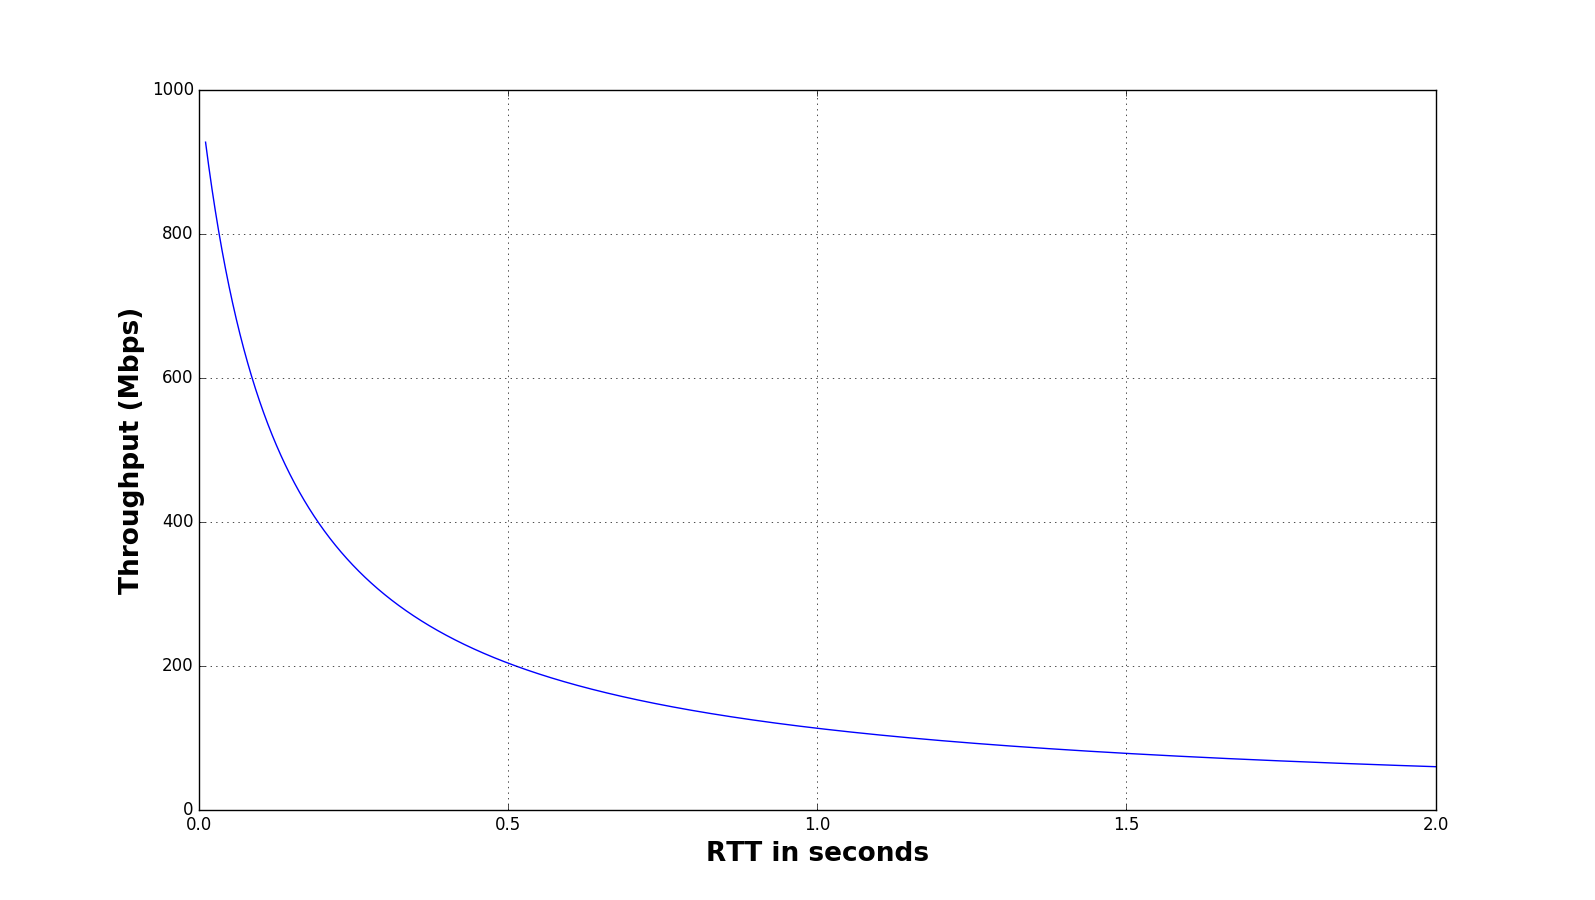
\includegraphics[width=150mm]{acn_ass_1}
    \caption{Throughput V/S RTT}
\end{figure}
\newline \newline
\bigskip

\textbf{Solution 4}\\
\begin{itemize}
\item In the first if we consider the case of without segmentation total time taken from Source to Destination would be three time of time taken from source to packet switch 1 as all the links have the same speed and thus
\begin{center}
Time = $\dfrac{3*7.5*10^6}{1.5*10^6}$ \\
\leavevmode \newline
Time = 15s
\end{center}
\item In the second case, time taken for a packet to reach from source to first packet switch would be following 
\begin{center}
Time = $\dfrac{1500}{1.5*10^6}$ \\
\leavevmode \newline
Time = 1ms
\end{center}
\item In the third case, time taken for a file to reach from source to destination considering fragmentation would be following
\begin{center}
Time = $\dfrac{3*1500}{1.5*10^6} + \dfrac{7.5*10^6-1500}{1.5*10^6}$ \\
\leavevmode \newline
Time = 5002 ms
\end{center}
\end{itemize}
\bigskip

\textbf{Solution 5}\\ \\
\textbf{Part a} \\
Some sender can create more than one flow as compared to some sender who is just creating one flow. In that case sender 1 has an advantage over sender 2 by creating more flows
In the figure 2 sender(s1) creates two flows for the same request while sender(s2) creates only one flow and then according to flow fairness we violate per-sender fairness.
\begin{figure}[h!]
    \centering
    \includegraphics[width=80mm]{acn_ass1}
    \caption{Flow Fairness v/s Per-user fairness}
\end{figure}

\textbf{Part b} \\
Network support seems like an obvious requirement because someone has to know which flow is coming from which sender and thus after that apply proper rules and regulations on it.
\clearpage

%=======================================

\end{document}